
\documentclass{beamer}

\mode<presentation> {

\usetheme{Madrid}

}

\usepackage{graphicx} 
\usepackage{booktabs} 
\usepackage[italian]{babel}
%----------------------------------------------------------------------------------------
%	TITLE PAGE
%----------------------------------------------------------------------------------------

\title[Relazione progetto finale]{Sistema cloud based per la gestione real-time di eventi geolocalizzati}

\author{Francesco Di Franco} % Your name
\institute[UniCT] 
{
Univerist\`a degli studi di Catania \\ % Your institution for the title page
\medskip
\textit{} 
}
\date{09-03-2016} 

\begin{document}
%SLIDE 1  Buongiorno sono francesco di franco e  presento la tesi "Sistema cloud ...."
\begin{frame}
\begin{table}[]
\centering
\begin{tabular}{ll}

\begin{minipage}{0.4\textwidth}
\begin{center}

\includegraphics[scale=0.15]{../img/logo_unict.png}
\end{center}
\end{minipage}

&  
\begin{minipage}{0.5\textwidth}


\includegraphics[scale=0.07]{../img/logoPSM.png}

\end{minipage}

\end{tabular}
\end{table}
\titlepage
\end{frame}


%SLIDE 2 La tesi è stata svolta nell'ambito del progetto aziendale perksmart. Il prodotto tramite telecamere installate a bordo strada riesce a guidare i propri utenti allo stallo di parcheggio libero più vicino.
\begin{frame}
\frametitle{Park Smart}
Parksmart 
\begin{itemize}
\item Software di videoanalisi
\item Sistema software per la gestione real-time di eventi
\item Applicazione per smartphone
\end{itemize}
\end{frame}

%SLIDE 3 Per lo sviluppo di questo progetto sono state usate le tecnologie cloud di amazon web services. Grazie a tali teconologie è stato risoloto il problema della scalabilità orizzantale delle risorse. Nello specifico sono state usate:

\begin{frame}
\frametitle{Amazon web services}
\begin{columns}[c] 

\column{.45\textwidth} 

\begin{enumerate}
\item ElasticBeanstalk
\item ElasticCache
\item Cognito
\item DynamoDB
\end{enumerate}

\column{.5\textwidth} 
Per lo sviluppo di questo progetto sono state usate le tecnologie cloud di Amazon web services. Grazie ai servizi SaaS usati \`e stato risolto il problema della scalabilit\`a orizzontale delle risorse.

\end{columns}
\end{frame}


%SLIDE 4 I componenti del sistema real time sono: un applicazione in nodejs, framework javascript a eventi che estende l'architettura rest. Un database dynamoDb, tecnologia Nosql propietaria amzon, un modulo web-socket implementato tramite socket.io, e database in redis, all in memory key value store usata come cache lru di supporto.    

\begin{frame}
\frametitle{Componenti sistema real time}
\begin{block}{NodeJs}
Un framework Javascript a eventi che estende l'architettura REST (Http). 
\end{block}

\begin{block}{DynamoDb}
Tecnologia di DBMS NoSql propietaria Amazon.
\end{block}

\begin{block}{Socket.io}
Libreria molto flessibile che implementa web-socket.
\end{block}

\begin{block}{Redis}
Tecnologia di DBMS NoSql, all in memory key-value store usata come cache di supporto.
\end{block}
\end{frame}



%SLIDE 5 Adesso vedremo il processo di autenticazione utilizzato:.
% L'utente, dopo aver effettuato il login su un identity provider, e aver ottenuto un token con validità temporale avrà accesso alle risorse.

\begin{frame}
\frametitle{Autenticazione}
\centerline{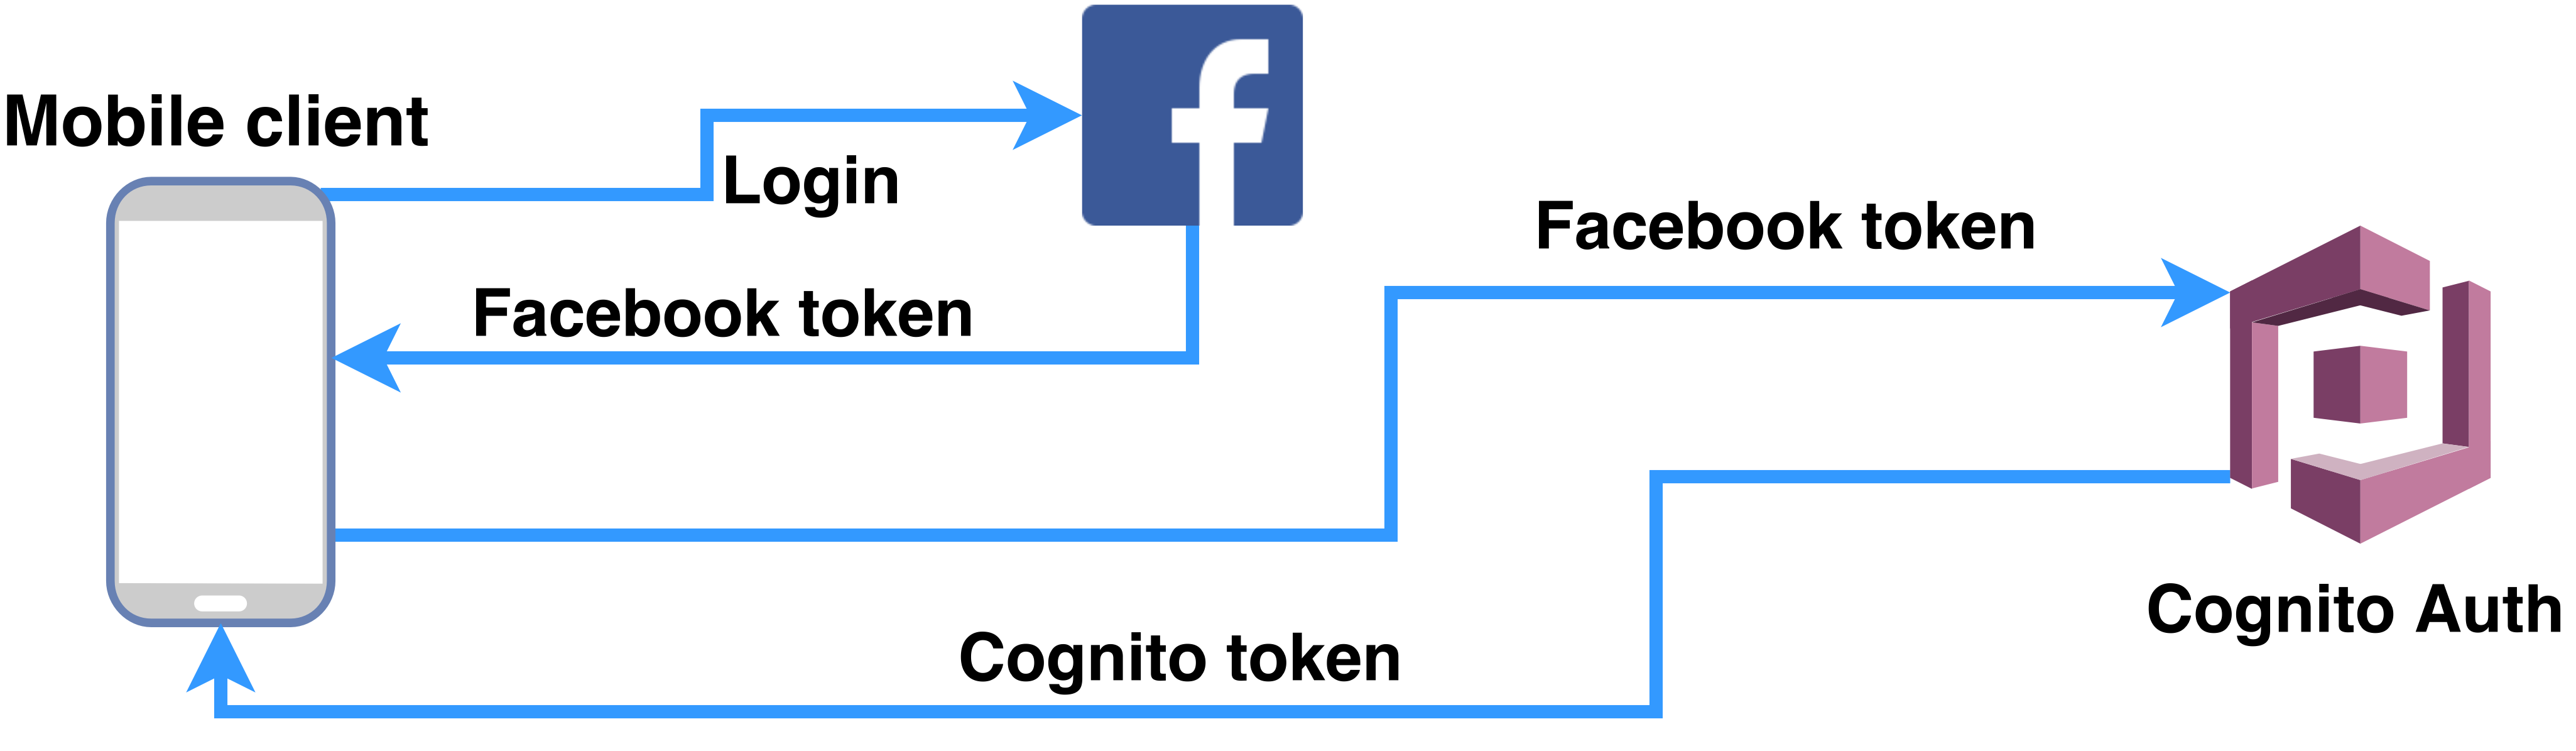
\includegraphics[scale=0.07]{../img/mobile_auth.png}}
\end{frame}


%Fornendo il token ottenuto e la posizione gps occupata l'utente potrà richiedere i dati per la relativa area geografica e potrà aprire una comunicazione web socket per rimanere in ascolto su eventi in prossimità della sua posizione. 
\begin{frame}
\frametitle{Container e load balancing}
\centerline{\includegraphics[scale=0.5]{../img/elastic.png}}
\end{frame}

%Ad ogni richiesta l'applicazione interrogherà la cache LRU, in caso di cache miss verrà interroganto il database, grazie a tale tecnica si si riducuno le effettive richieste al database aumentando il througput.
\begin{frame}
\frametitle{Cache hit/miss}
\centerline{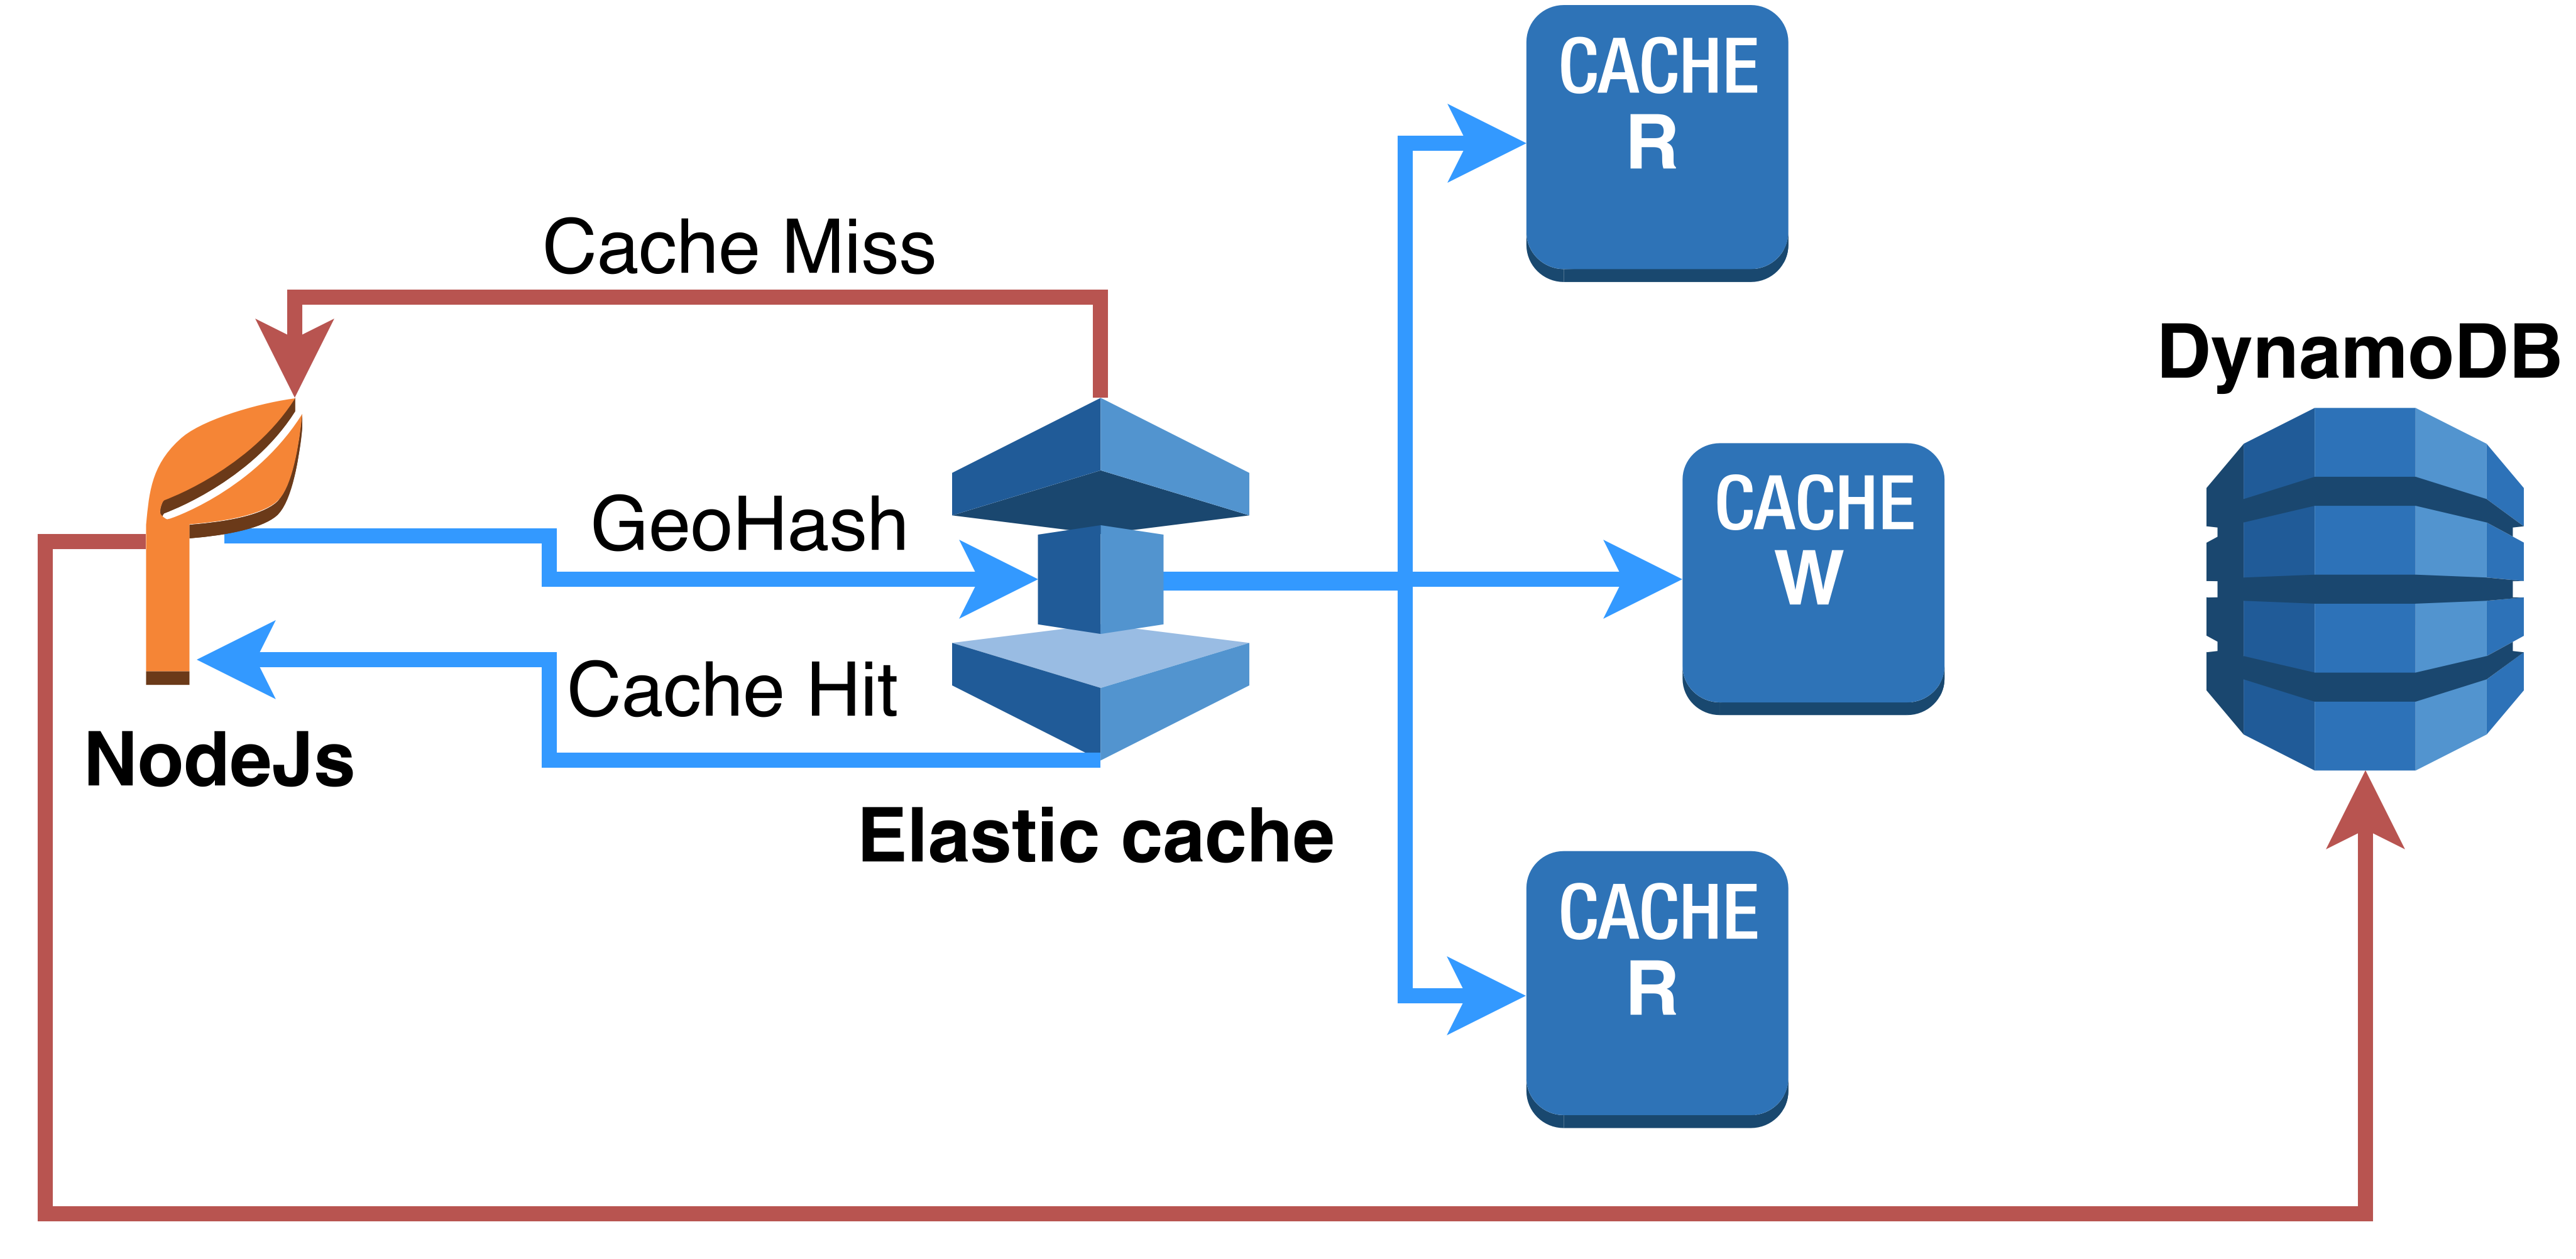
\includegraphics[scale=0.07]{../img/DataFetch.png}}
\end{frame}


%Tale cache svolge un altro ruolo fondamentale. Grazie al meccanismo del publish/subscribe ogni istanza nodejs potrà rimanere in ascolto per eventuali aggiornamenti.
\begin{frame}
\frametitle{Publish/Subscribe}
\centerline{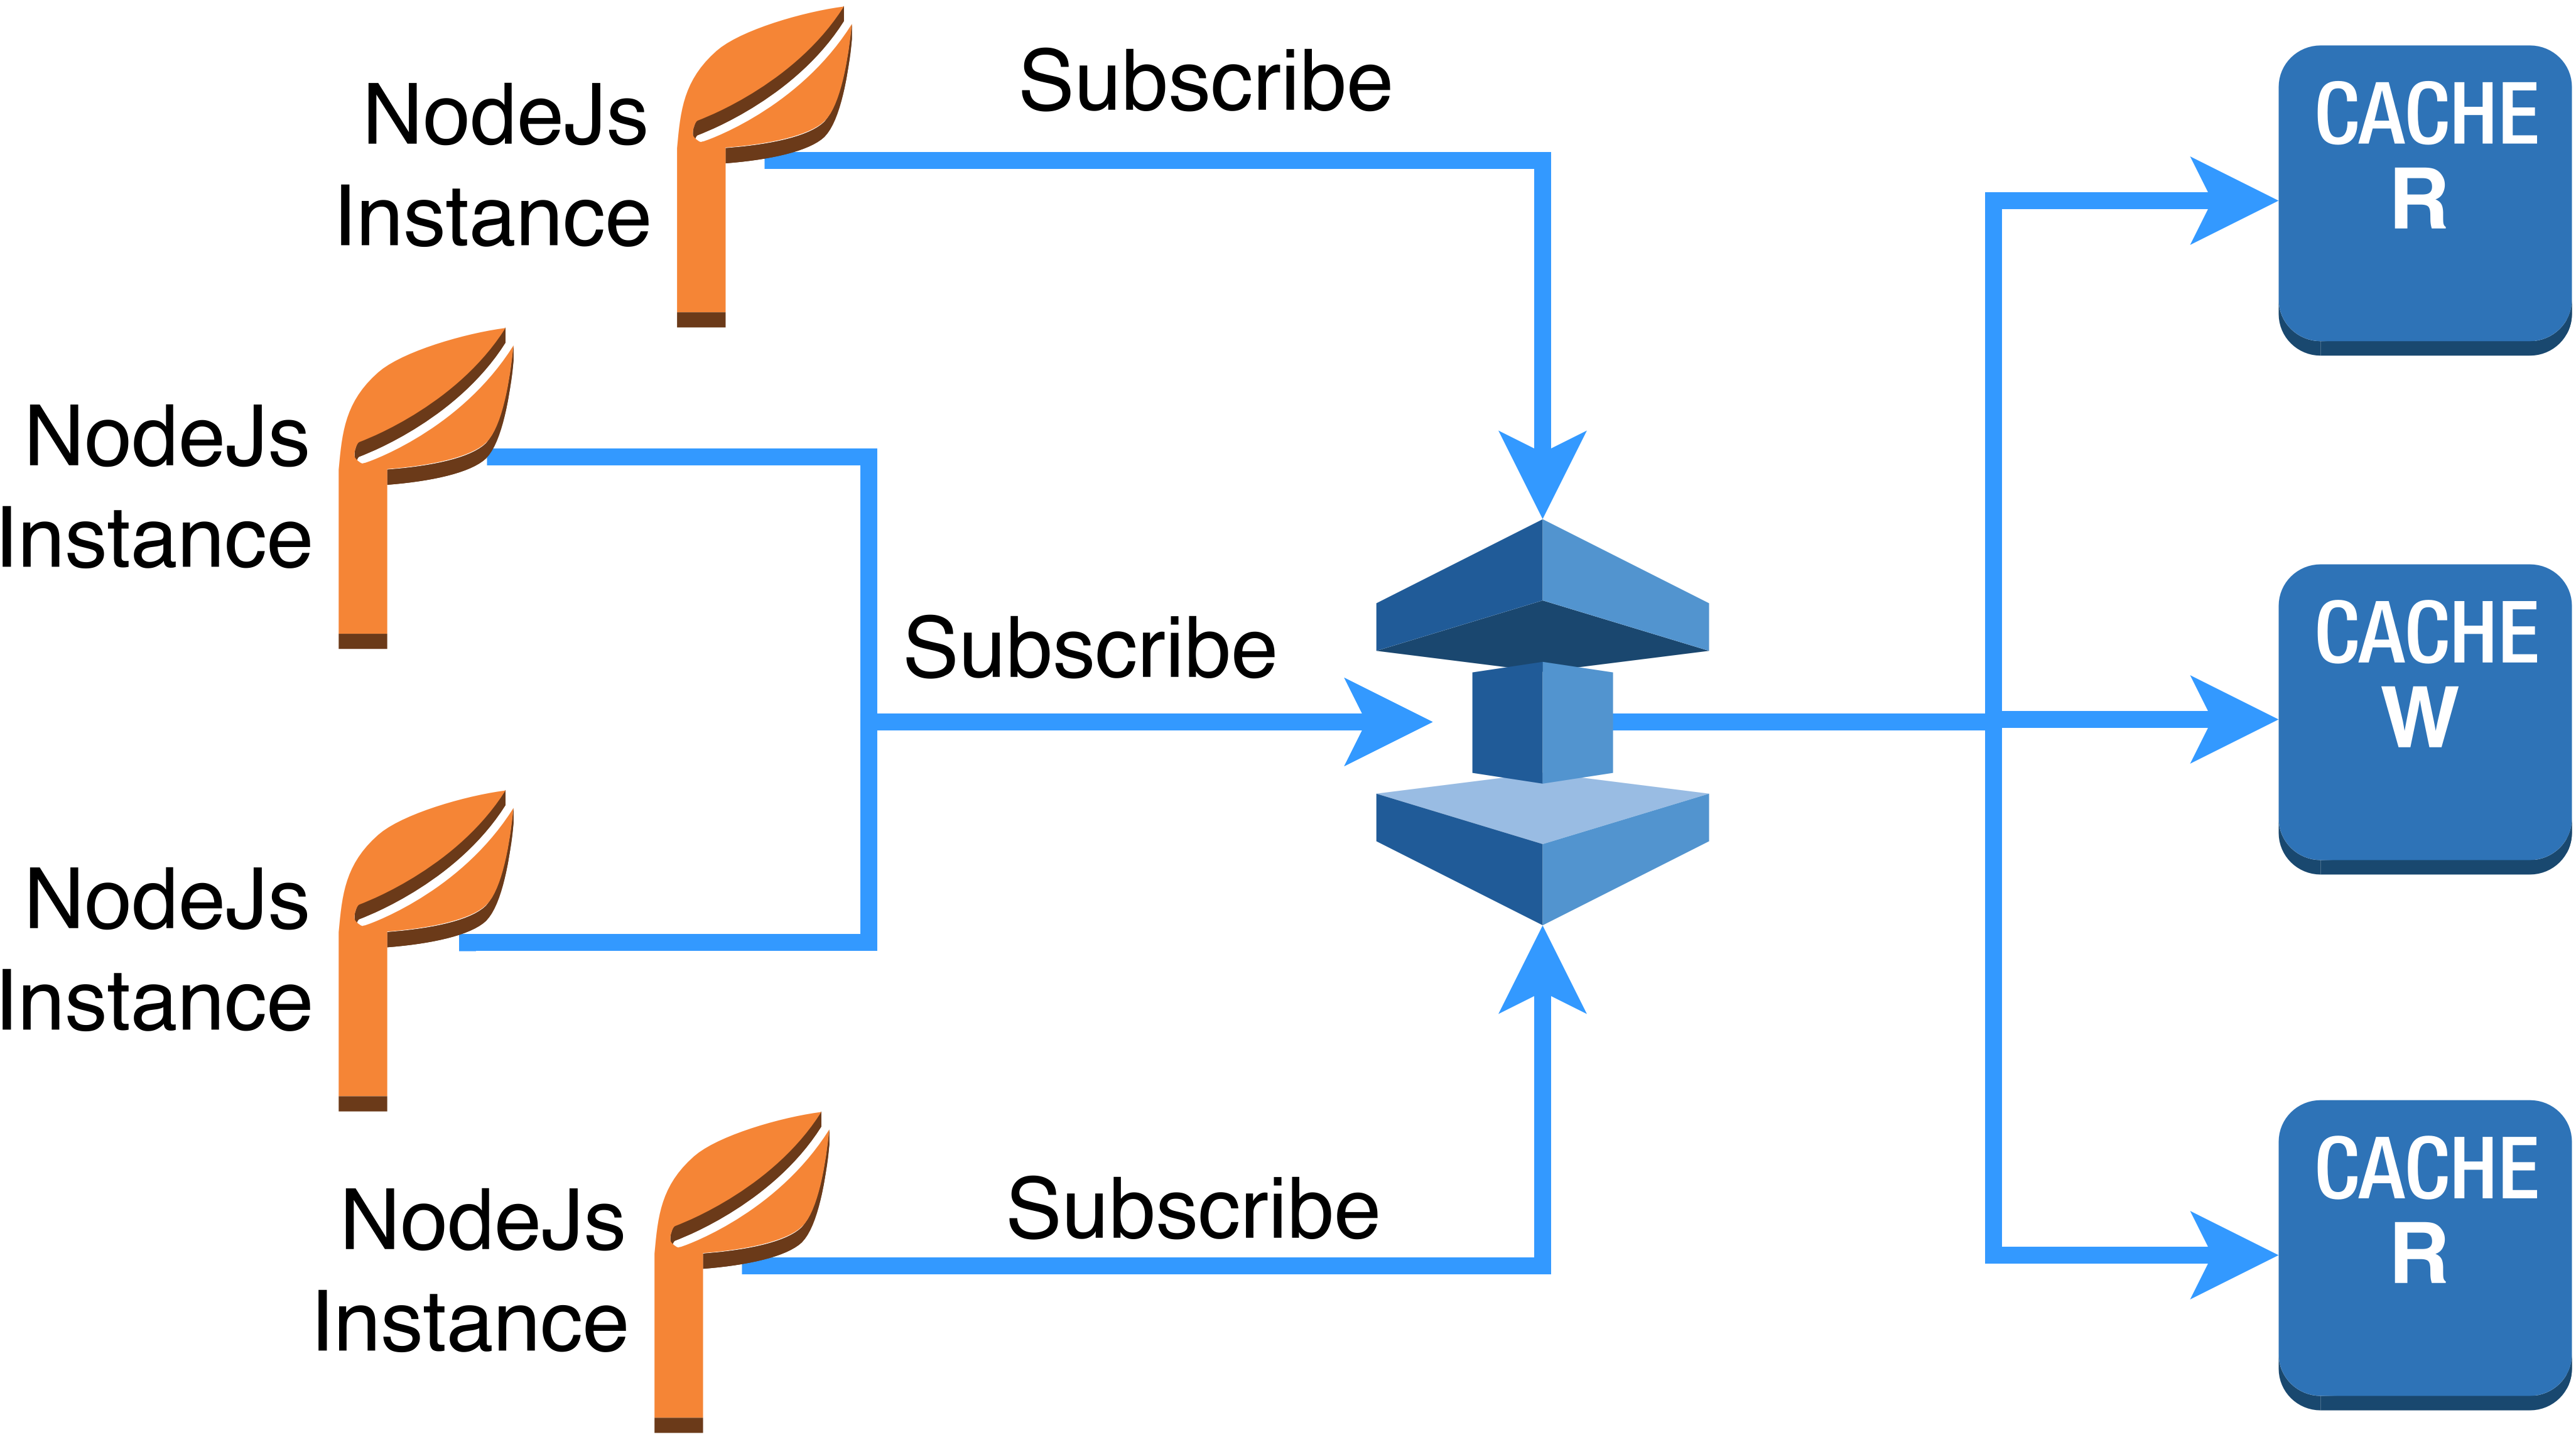
\includegraphics[scale=0.07]{../img/subscribe.png}}
\end{frame}

%Quando una videocamera rileva il camabio di stato di uno stallo di parcheggio notificherà l'evento al cloud. Tale notifica verrà gestita da una delle n istanze presenti nell'auto scaling group. Alla ricezione di tale aggiornamento si effettuerà un publish sulla cache che notificherà tutte le istanze in ascolto.
\begin{frame}
\frametitle{Websocket notification}
\centerline{\includegraphics[scale=0.08]{../img/updateps.png}}
\end{frame}


%Di conseguenza ogni istanza, consapevole dell'evento, si occuperà di notificare tutti gli utenti in prossimità dell'evento stesso
\begin{frame}
\frametitle{Mobile notification}
\centerline{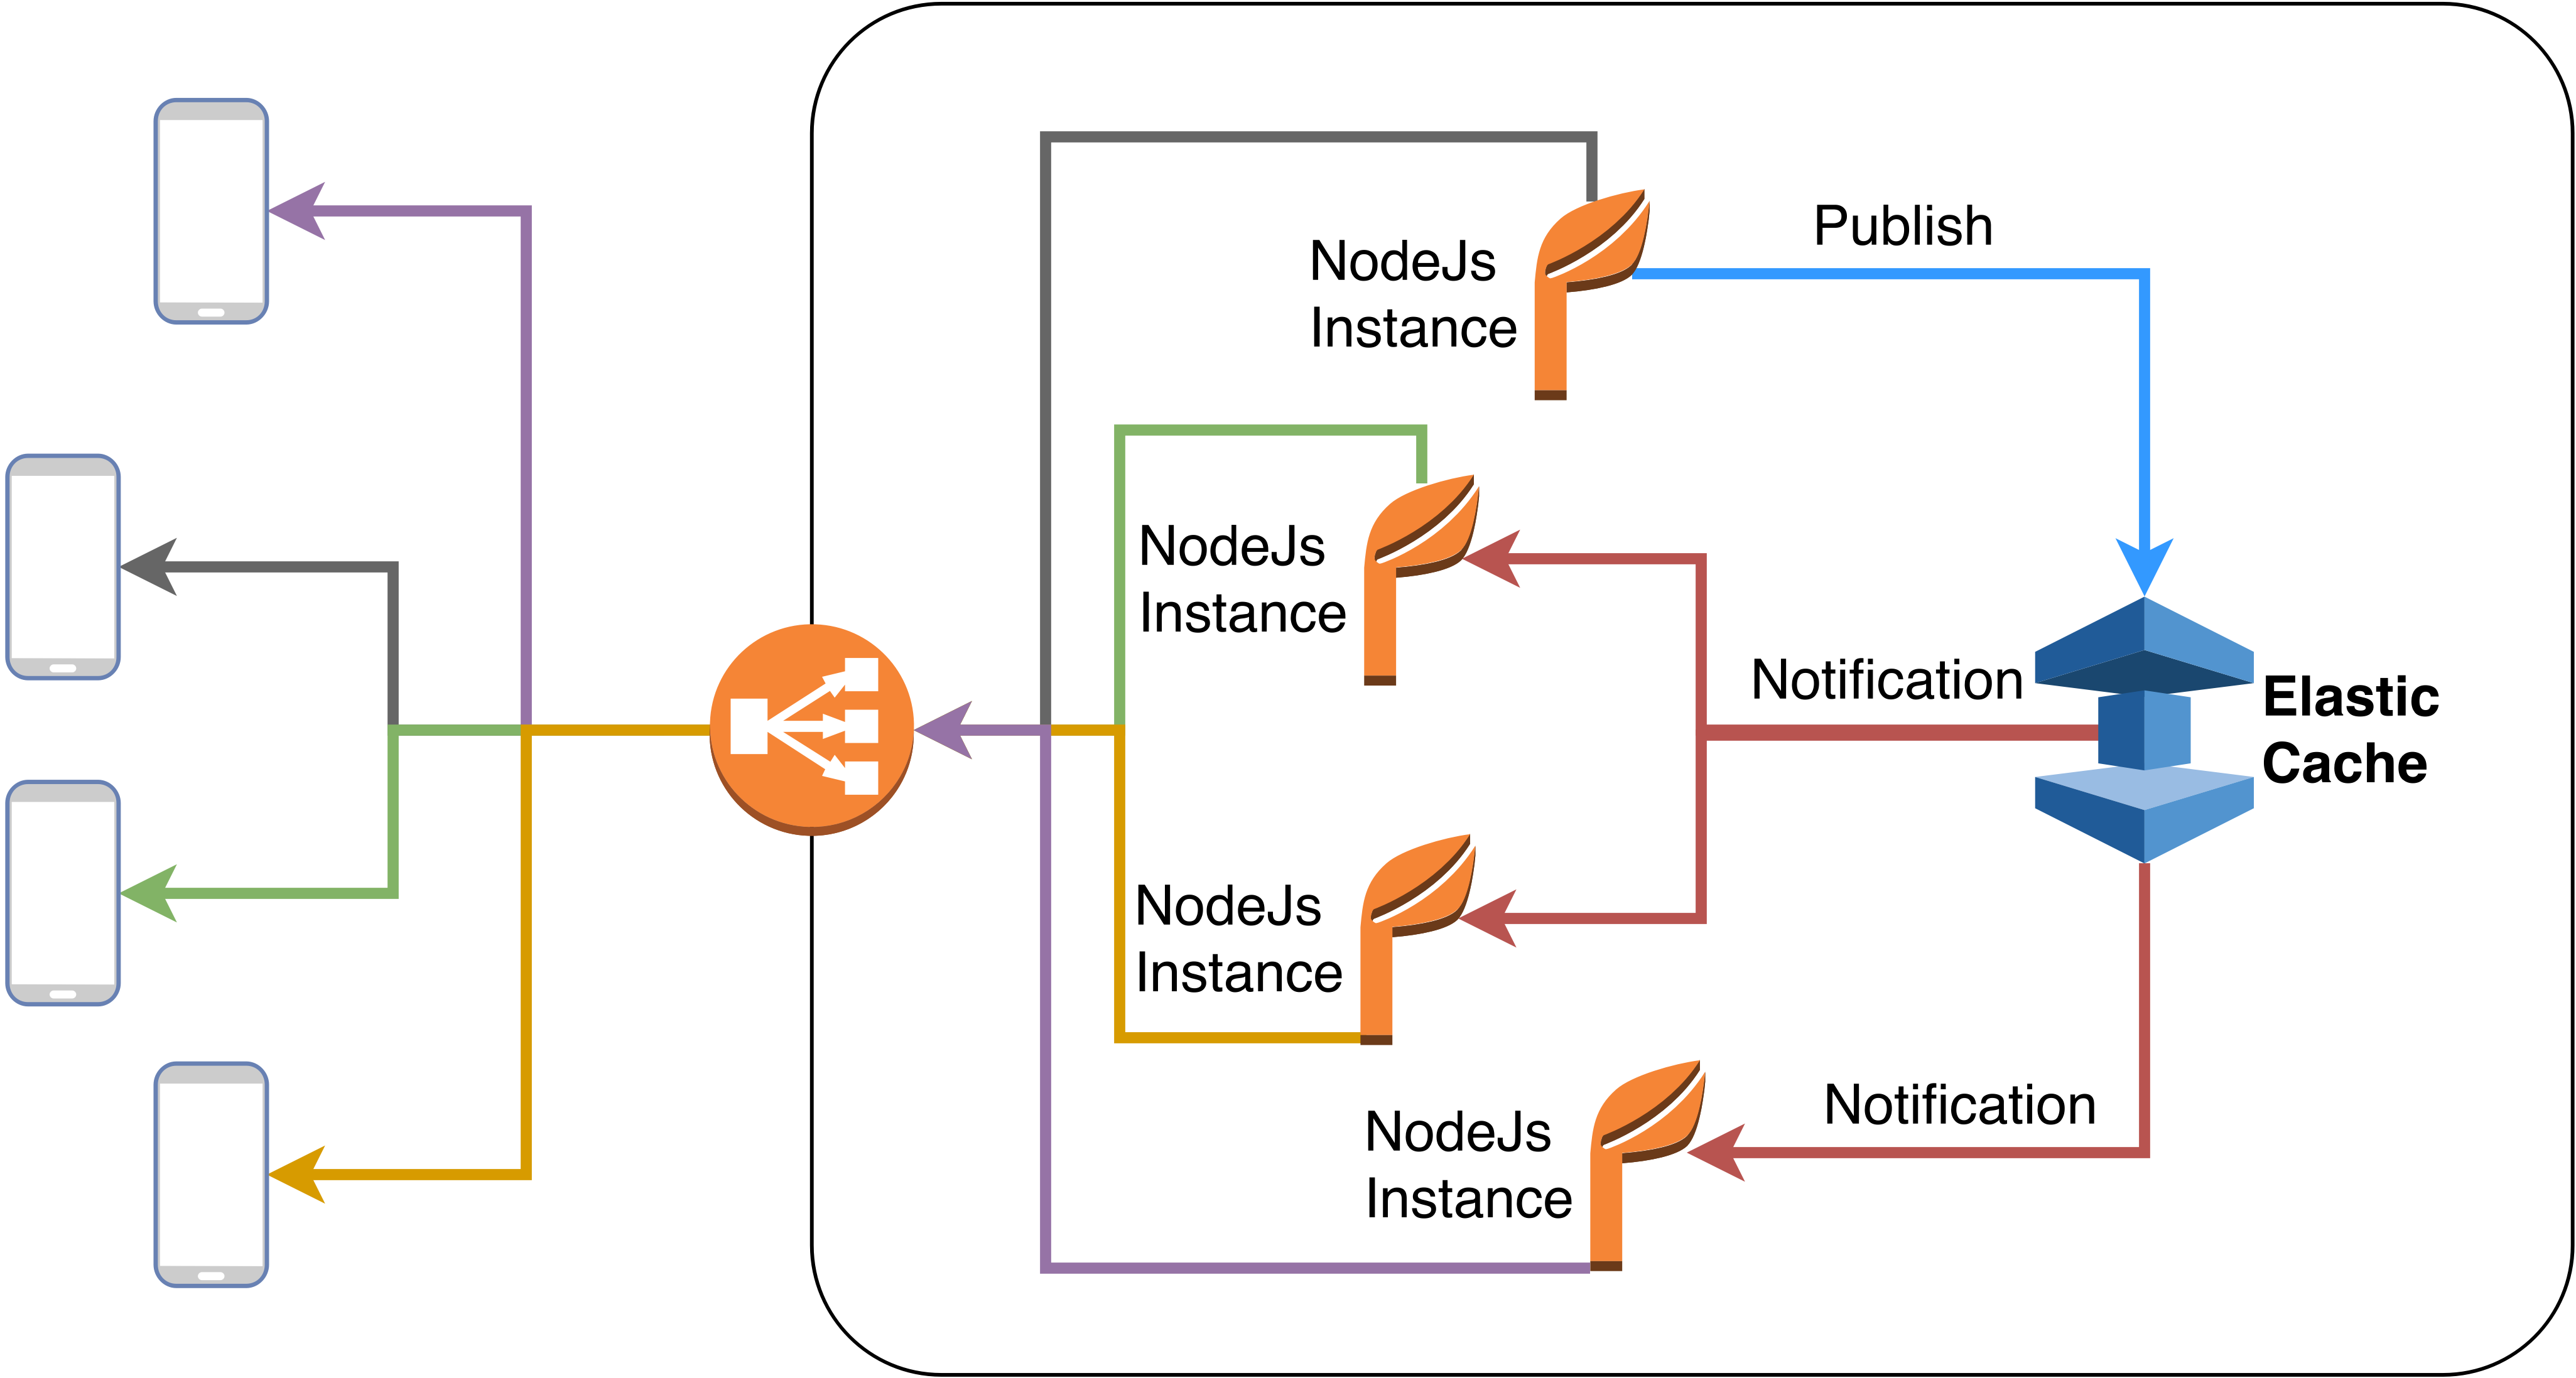
\includegraphics[scale=0.08]{../img/notification.png}}
\end{frame}





%SLIDE 5
\begin{frame}
\Huge{\centerline{The End}}
\end{frame}

%----------------------------------------------------------------------------------------

\end{document}
